\documentclass[11pt,a4paper]{article}
\usepackage[utf8]{inputenc}
\usepackage[T1]{fontenc}
\usepackage[spanish,es-nodecimaldot]{babel}
\usepackage{amsmath,amssymb,bm,booktabs,graphicx,geometry}
\usepackage[colorlinks=true,allcolors=blue]{hyperref}
\geometry{margin=24mm}
\graphicspath{{results/K5_target_20260927_130037_245/}}
\title{Diseño de inclinación con cinco orientaciones\\\large Cobertura de PEB de 10 cm, $m_R=1.9$ y conocimiento angular incierto}
\author{Proyecto Cambridge}
\date{27 de septiembre de 2026}
\begin{document}
\maketitle
\begin{abstract}
Se busca una inclinación común para cinco normales de un PD reorientable que maximice la fracción del dominio con PEB tridimensional no mayor que 10 cm. Se compara conocimiento perfecto de las orientaciones con incertidumbre de medida de un grado por componente angular, usando una FIM ampliada que elimina las poses como parámetros auxiliares. El barrido no optimiza individualmente los diez grados de libertad de las cinco normales: se restringe a un cono uniforme de inclinación común. Se distingue el máximo de cobertura, la menor inclinación que satisface una cobertura absoluta del 95\%, y la menor inclinación situada a un punto porcentual del máximo. Se explican el protocolo de sensibilidad, el papel de la FOV y las limitaciones de una cota local.
\end{abstract}
\tableofcontents

\section{Configuración fija y variables del estudio}
\begin{center}
\begin{tabular}{ll}
\toprule
Parámetro & Valor \\
\midrule
Posición del LED & $(0,0,2.5)$ m \\
Eje del LED & $(0,0,-1)$ \\
Potencia óptica & 0.65 W \\
Semiángulo LED / orden emisor & $45^\circ$ / $m_T=2$ \\
Área del PD & $75.4\ \mathrm{mm}^2$ \\
Orden receptor & $m_R=1.9$ \\
FOV del receptor & $46^\circ$ de semiángulo, corte duro \\
Número de orientaciones & $K=5$ \\
Muestras por orientación & $N_i=1000$, total 5000 \\
Ruido por muestra & $3\times10^{-14}\ \mathrm W^2$ \\
Dominio evaluado & $[-1,1]\times[-1,1]\times[0,1.4]\ \mathrm m^3$ \\
Barrido de inclinación & $0:0.25:85$ grados \\
Desviación estándar angular & $0^\circ$ y $1^\circ$ por componente \\
\bottomrule
\end{tabular}
\end{center}
El recinto nominal mide $2\times2\times2.5$ m, pero el receptor se evalúa hasta $z=1.4$ m; no se afirma cobertura en la parte superior no muestreada. Se mantiene ruido óptico independiente y homoscedástico, ganancia calibrada y centro óptico sin traslación durante el barrido.

Los azimuts son $\alpha_i=72^\circ(i-1)$, $i=1,\ldots,5$, y las normales de cada configuración son:
\begin{equation}
 \mathbf n_i(\theta)=[\sin\theta\cos\alpha_i,\sin\theta\sin\alpha_i,\cos\theta]^{\mathsf T}.
\end{equation}
El mismo conjunto se usa en todas las posiciones, sin orientar el PD desde la posición verdadera. El ángulo óptimo de este informe es el del barrido discreto de esta familia, con este offset azimutal, FOV, potencia, área y presupuesto; no un óptimo global de codebooks 2DoF.

\section{Definición de cobertura y criterio de selección}
Sea $\mathcal R_h$ la rejilla espacial. Para $\tau=0.10$ m:
\begin{equation}
 \rho_{\tau}(\theta)=\frac1{|\mathcal R_h|}\sum_{\mathbf r\in\mathcal R_h}
 \mathbf1\{\operatorname{isfinite}(\mathrm{PEB}(\mathbf r;\theta)),\ \mathrm{PEB}(\mathbf r;\theta)\leq\tau\}.
\label{eq:coverage}
\end{equation}
Se utiliza $\leq$, coherente con el parámetro de cobertura solicitado. El denominador incluye todos los puntos, también los no identificables y las fronteras excluidas. Se guarda además la cobertura regular:
\begin{equation}
 \rho_{\rm reg}(\theta)=|\mathcal R_h|^{-1}\sum_{\mathbf r\in\mathcal R_h}\mathbf1\{\mathrm{PEB}\ \text{finito y regular}\}.
\end{equation}
Ninguna de estas cantidades es la probabilidad de que un error estimado sea menor que 10 cm. Una cota pequeña es una condición favorable, no garantía de precisión alcanzada por un estimador sesgado o por hardware mal calibrado.

Se consideran tres decisiones distintas:
\begin{align}
 \theta_{\rm max}&=\min\arg\max_{\theta\in\Theta_h}\rho_\tau(\theta),\\
 \theta_{95}&=\min\{\theta\in\Theta_h:\rho_\tau(\theta)\geq0.95\},\\
 \theta_{\rm cerca}&=\min\{\theta\in\Theta_h:\rho_\tau(\theta)\geq\max_{\vartheta}\rho_\tau(\vartheta)-0.01\}.
\end{align}
Se elige la menor inclinación en caso de empate exacto de cobertura. El 95\% define aquí ``aceptable'' y la pérdida de un punto porcentual define ``cerca del máximo'': son decisiones explícitas y editables, no constantes físicas. Si no existe $\theta_{95}$ se devuelve \texttt{NaN}, no el mejor candidato etiquetado falsamente como viable.

La rejilla de diseño tiene 968 puntos (paso 0.2 m); la de comprobación tiene 6615 (paso 0.1 m). Se evalúan todas las inclinaciones en ambas. El archivo \texttt{grid\_agreement.csv} añade el menor tilt que cumple el requisito absoluto en las dos rejillas y el menor que queda a un punto porcentual del máximo de \emph{cada} una. Esto no constituye una certificación sobre el volumen continuo.

\section{Cómo entra el error de un grado en el PEB}
\subsection{No es un cambio arbitrario del ruido RSS}
La curva con $1^\circ$ utiliza \texttt{rx\_pose\_error\_peb}. El modelo de potencia nominal es:
\begin{equation}
 \mu_i=\beta s_i^\nu,\quad \nu=1.9,\quad s_i=\mathbf n_i^{\mathsf T}\mathbf u,\quad
 \beta=Cf_T(\mathbf u)/d^2.
\end{equation}
Cada normal verdadera se parametriza localmente por dos coordenadas angulares desconocidas $\boldsymbol\delta_i$. Se dispone de una medida de pose $\hat{\boldsymbol\delta}_i=\boldsymbol\delta_i+\mathbf e_i$, donde:
\begin{equation}
 \mathbf e_i\sim\mathcal N(0,\sigma_\theta^2I_2),\qquad
 \sigma_\theta=\frac\pi{180}\ \mathrm{rad}.
\end{equation}
El punto verdadero del análisis es $\boldsymbol\delta_i=0$ respecto a las normales nominales. Es un punto de evaluación de parámetros auxiliares desconocidos, no una información entregada al estimador.

Con $E_i$ una base ortonormal tangente a $\mathbf n_i$, la derivada RSS respecto a su pose es:
\begin{equation}
 D_{i,\{2i-1,2i\}}=\beta\nu s_i^{\nu-1}\mathbf u^{\mathsf T}E_i.
\end{equation}
Si $J$ es el Jacobiano cartesiano de posición, $\Sigma_y=\operatorname{diag}(\sigma^2/N_i)$ y $\Sigma_\theta=\sigma_\theta^2 I_{2K}$, la FIM ampliada es:
\begin{equation}
 I=\begin{bmatrix}
 J^{\mathsf T}\Sigma_y^{-1}J&J^{\mathsf T}\Sigma_y^{-1}D\\
 D^{\mathsf T}\Sigma_y^{-1}J&D^{\mathsf T}\Sigma_y^{-1}D+\Sigma_\theta^{-1}
 \end{bmatrix}.
\end{equation}
Tras eliminar las poses mediante el complemento de Schur:
\begin{equation}
 I_e=J^{\mathsf T}(\Sigma_y+D\Sigma_\theta D^{\mathsf T})^{-1}J,\qquad
 \mathrm{PEB}_{\rm pose}=\sqrt{\operatorname{tr}(I_e^{-1})}.
\label{eq:efim}
\end{equation}
Así, \textbf{sí se incorpora el grado de incertidumbre en la CRLB/PEB}, no sólo en simulaciones de estimadores. Para errores independientes, el término angular equivalente es diagonal:
\begin{equation}
 [D\Sigma_\theta D^{\mathsf T}]_{ii}=\sigma_\theta^2\beta^2\nu^2s_i^{2\nu-2}(1-s_i^2).
\end{equation}
La implementación vectorizada es algebraicamente equivalente al complemento de Schur original y se contrasta con él en pruebas. Los puntos de frontera siguen excluidos y los rangos deficientes conservan PEB infinito.

\subsection{Interpretación exacta de la unidad}
El campo editable es \texttt{experiment.orientation\_std\_deg=1}. Al llamar al núcleo se pasa su cuadrado, porque éste recibe varianza en grados cuadrados. Para un valor $a$, se usa $a^2(\pi/180)^2$ como varianza por componente tangente. No debe cambiarse directamente esa conversión a $a(\pi/180)^2$.

Un grado por componente no significa que la rotación total esté acotada por un grado: para pequeños errores, su RMS es aproximadamente $\sqrt2$ grados. Tampoco equivale a imponer un grado de error a cada coordenada cruda de inclinación y azimut; la sensibilidad del azimut contiene $\sin\theta$. Si el objetivo fuera RMS total de normal de $1^\circ$, el parámetro isotrópico por componente sería aproximadamente $1/\sqrt2$ grados.

\subsection{Qué protocolo no se está usando}
La cota no supone que se perturban normales y luego se entregan al algoritmo como perfectamente conocidas. Eso correspondería a otro diseño con información de oráculo y podría mejorar diversidad angular. Tampoco se modela aquí como principal un jitter de actuación no observado con prior marginal. Ese otro experimento está en \path{../Reorientation sensitivity/sim02_actuation_error.m} y su cota de momentos es aproximada. El informe \path{../Reorientation sensitivity/Sensitivity_report.tex} distingue ambos modelos y el error común de actitud.

\section{Resultados del barrido}
\begin{center}\small
\begin{tabular}{lrrrr}
\toprule
Rejilla / $\sigma_\theta$ & Máximo & $\theta_{\rm max}$ & $\theta_{95}$ & $\theta_{\rm cerca}$ \\
\midrule
Diseño / $0^\circ$ & 97.521\% & $3.5^\circ$ & $2.25^\circ$ & $2.75^\circ$ \\
Comprobación / $0^\circ$ & 98.579\% & $4.25^\circ$ & $2^\circ$ & $2.25^\circ$ \\
Diseño / $1^\circ$ & 86.364\% & $25.75^\circ$ & No existe & $24.25^\circ$ \\
Comprobación / $1^\circ$ & 89.751\% & $25.5^\circ$ & No existe & $23^\circ$ \\
\bottomrule
\end{tabular}
\end{center}
Sin incertidumbre de pose, el tilt de $2.25^\circ$ supera el requisito del 95\% en ambas rejillas: 96.074\% en diseño y 97.793\% en comprobación. Es una recomendación de baja inclinación distinta del máximo de cobertura. Con $1^\circ$ por componente, ese mismo tilt sólo cubre aproximadamente 4.641\% de la rejilla densa bajo el umbral de 10 cm; no puede mantenerse la recomendación ideal ignorando incertidumbre angular.

Con incertidumbre, $23^\circ$ logra 88.904\% en la rejilla densa, frente al máximo 89.751\% a $25.5^\circ$. Si se exige estar a menos de un punto porcentual del máximo en ambas rejillas, el menor tilt es $24.25^\circ$: 85.950\% en diseño y 89.599\% en comprobación. Esto es un compromiso cercano al mejor caso ensayado, \emph{no} cumplimiento del objetivo absoluto del 95\%.

El máximo denso con incertidumbre presenta 91.504\% de cobertura regular, pero sólo 89.751\% de cobertura de PEB objetivo. Su RMS condicionado a posiciones finitas es 5.583 cm; el RMS sobre todo el dominio sigue siendo infinito por los puntos no identificables. No se sustituye ese infinito por el promedio favorable del subconjunto.

La diferencia entre rejillas es visible, especialmente con incertidumbre (unos 3.39 puntos porcentuales entre máximos). Por ello no se declara convergencia espacial ni un óptimo continuo. El ángulo se ensaya en pasos de $0.25^\circ$, no se prueba optimalidad entre muestras angulares.

\begin{figure}[htbp]\centering
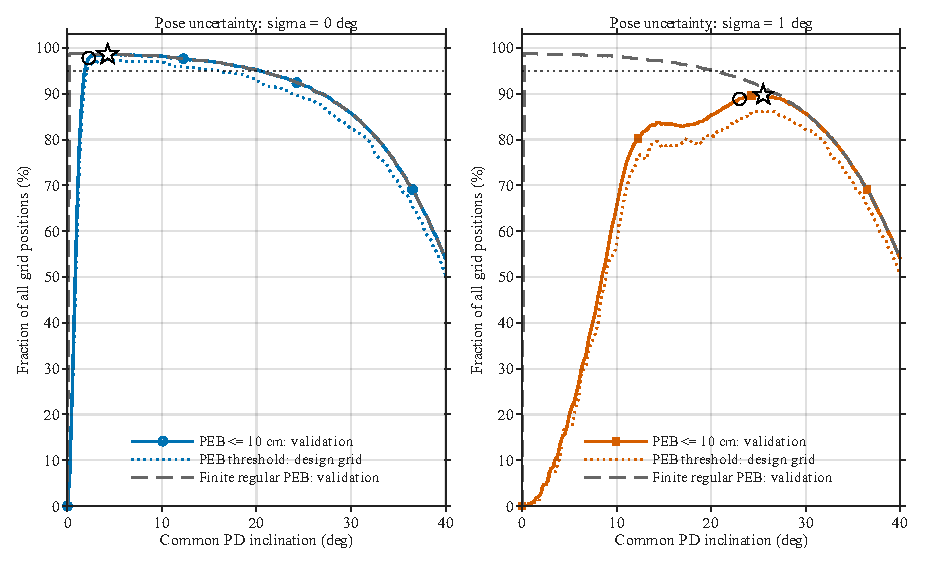
\includegraphics[width=0.96\linewidth]{Target_tilt_coverage.pdf}
\caption{Cobertura regular y cobertura bajo 10 cm. La estrella señala el primer máximo en la rejilla densa y el círculo negro la menor inclinación a un punto porcentual del máximo. La horizontal punteada marca 95\%. Se muestra hasta $40^\circ$ para legibilidad; el barrido guardado llega a $85^\circ$.}
\end{figure}
\begin{figure}[htbp]\centering
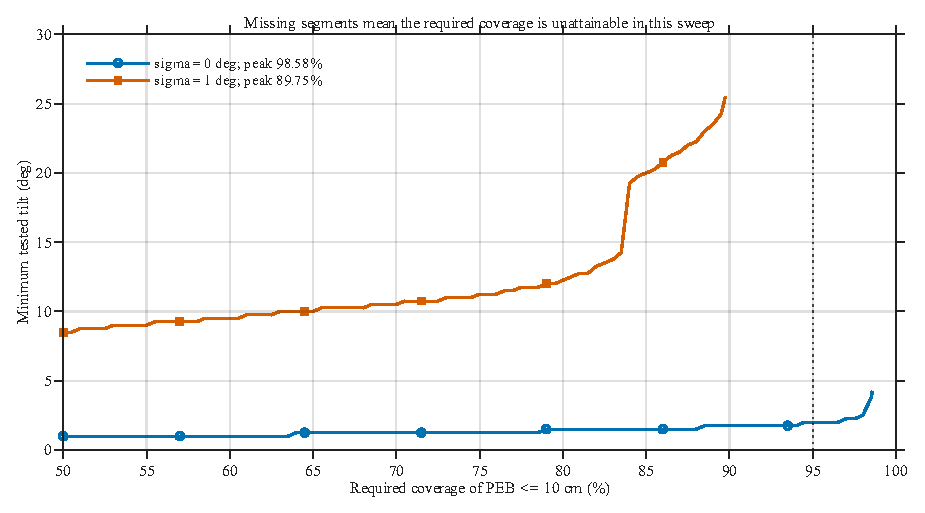
\includegraphics[width=0.96\linewidth]{Minimum_tilt_for_coverage.pdf}
\caption{Menor inclinación ensayada para distintos requisitos absolutos de cobertura. Los requisitos no alcanzables no se extrapolan.}
\end{figure}
\begin{figure}[htbp]\centering
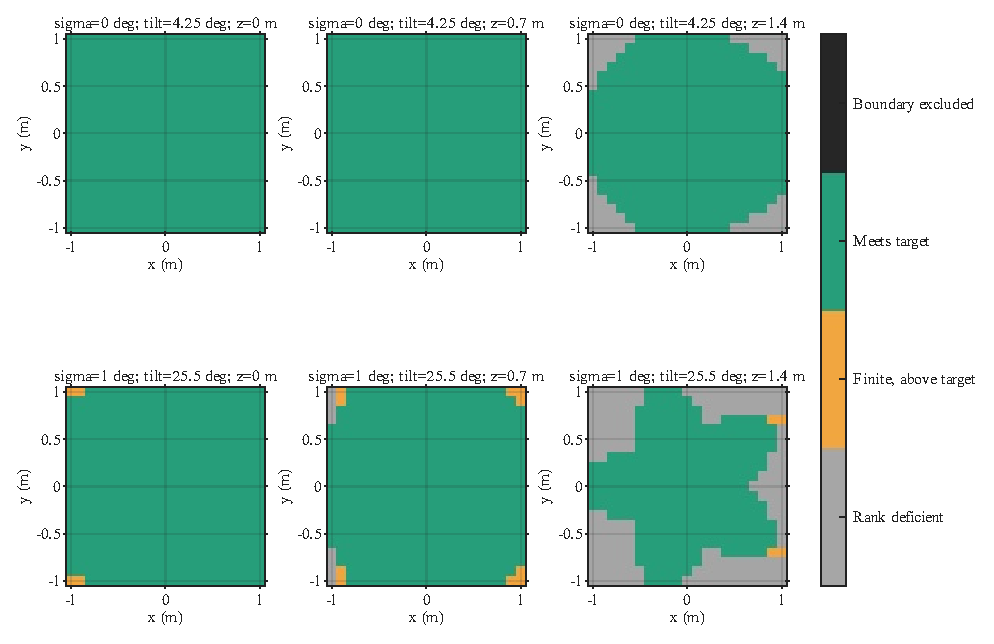
\includegraphics[width=0.98\linewidth]{Selected_tilt_spatial_coverage.pdf}
\caption{Mapas de clases en las configuraciones de máxima cobertura densa, con distintas alturas. Verde: cumple 10 cm; naranja: finito pero excede el umbral; gris: rango insuficiente; oscuro: frontera excluida. Cada fila utiliza su inclinación seleccionada, no un ángulo común entre modelos.}
\end{figure}

\section{Explicación de la tendencia y del compromiso}
Con inclinación nula todas las normales coinciden y no existe identificabilidad 3D regular. Un aumento inicial de inclinación aporta contraste angular y reduce la cota; con orientaciones exactas bastan pocos grados para cumplir el umbral en buena parte del dominio.

Al incluir incertidumbre, un cono estrecho amplifica el efecto de errores de conocimiento angular sobre los pequeños contrastes entre observaciones. Un cono más amplio mejora ese condicionamiento, pero también hace salir observaciones de FOV y elimina posiciones donde quedan menos de tres normales independientes. La competencia entre precisión y aceptación geométrica produce el máximo alrededor de $25.5^\circ$ en la rejilla densa.

Esta optimización no permite mejorar arbitrariamente cobertura aumentando área o muestras: un punto fuera del soporte geométrico continúa fuera, y un régimen dominado por error de pose puede presentar un suelo de precisión. Para alcanzar 95\% con error de un grado habría que modificar otro recurso o modelo (por ejemplo aceptación angular, número/patrón de normales o precisión de pose) y volver a evaluar, no declarar viable el 89.75\%.

\section{Monte Carlo de auditoría: separado del mapa de cobertura}
Se ejecutan comparaciones de LS, GLS, WLS, NLS conjunto y NLS-TCOM en tres posiciones explícitas: $(0,0,0.6)$, $(0.25,-0.15,0.6)$ y $(-0.25,0.15,1.1)$ m, usando 300 ensayos por caso. Estas posiciones tienen visibilidad completa en los tilts seleccionados. No se escogen observaciones mediante una máscara de posición verdadera ni se pretende estimar con ellas la precisión de todo el recinto.

En cada ensayo, las potencias se generan con las normales verdaderas nominales; se añade ruido óptico con varianza $\sigma^2/N_i$. Se generan mediciones de pose ruidosas sobre la esfera y los estimadores reciben esas normales medidas, no las verdaderas. El error de orientación persiste durante todas las muestras ópticas de su orientación. Se utiliza la misma realización de RSS y pose para todos los métodos de un caso. Los estados de fallo se conservan.

La tabla \texttt{monte\_carlo\_points.csv} contiene RMSE, cota del punto, sesgo empírico, tasa de fallo y porcentaje de errores efectivos menores o iguales que 10 cm. Esta última columna es una probabilidad empírica por ensayo y \textbf{no} la cobertura espacial de \eqref{eq:coverage}. El NLS conjunto y el NLS-TCOM deben aproximarse cuando alcanzan el mismo mínimo, pero distintos solvers y tolerancias pueden dar estados numéricos distintos; no se fuerza identidad ocultando fallos.

La ejecución final contiene 210 filas método--caso (300 ensayos por fila), sin fallos registrados. A $\theta=25.5^\circ$ y $\sigma_\theta=1^\circ$, NLS conjunto y NLS-TCOM obtienen, respectivamente por posición, aproximadamente $3.035$, $3.115$ y $2.468$ cm de RMSE; las cotas de esos puntos son $3.048$, $3.091$ y $2.311$ cm. Las dos formulaciones NLS difieren como máximo $2.45\times10^{-7}$ cm en RMSE sobre la tabla completa. No se extrapola esa precisión puntual al volumen ni se confunde con su cobertura de cota.

\section{Advertencia física sobre FOV y media sensibilidad}
Para $m_R=1.9$, el ángulo que reduce la respuesta a la mitad es:
\begin{equation}
 \psi_{1/2}=\arccos(2^{-1/1.9})\approx46^\circ.
\end{equation}
Eso no implica señal cero fuera de $46^\circ$. Este estudio mantiene el valor actual de FOV como corte duro porque así está configurado el proyecto. Si los $46^\circ$ provienen únicamente de una especificación de media sensibilidad de la hoja de datos, deben separarse de la aceptación real antes de trasladar estos resultados a hardware. No se amplió FOV silenciosamente para obtener mejor cobertura.

\section{Cómo repetir y modificar el estudio}
\begin{verbatim}
addpath('CAMBRIDGE/simulations');
cambridge_setup();
sim01_K5_tilt_coverage;
\end{verbatim}
El script está en \path{Coverage target design}. Sus controles principales son:
\begin{verbatim}
p.receiver.m_R = 1.9;
p.design.coverage_threshold_cm = 10;
experiment.K = 5;
experiment.orientation_std_deg = 1;
experiment.minimum_coverage_percent = 95;
experiment.near_peak_loss_pp = 1;
\end{verbatim}
El umbral de cobertura global conserva \texttt{Inf} como valor por defecto en \texttt{system\_parameters}; sólo este experimento lo fija a 10 cm. Cambiarlo no recorta el PEB ni el RMS. Los criterios de viabilidad de sim05/sim07 mantienen además sus propios objetivos declarados, como \texttt{target\_peb\_m}.

Se guardan matrices PEB completas, parámetros, curvas CSV, decisiones de tilt, acuerdo entre rejillas y resultados Monte Carlo en un directorio con fecha. Para cambiar únicamente la presentación se usa \texttt{replot\_K5\_target\_results}; no se repite el cálculo de la FIM.

\section{Conclusiones operativas}
\begin{itemize}
\item Para orientaciones ideales, $2.25^\circ$ es una elección pequeña que cumple 95\% en ambas rejillas ensayadas; $4.25^\circ$ maximiza la cobertura densa.
\item Para incertidumbre de un grado por componente, ningún tilt ensayado alcanza 95\%. El máximo denso es 89.751\% a $25.5^\circ$; $24.25^\circ$ es el compromiso cercano al máximo de ambas rejillas.
\item El grado de error entra explícitamente en una CRLB con poses auxiliares. La simulación de estimadores es una comprobación distinta y restringida a puntos de visibilidad completa.
\item Estas conclusiones dependen de FOV, patrón, ganancia, ruido, calibración y dominio. No son garantías de error experimental ni de cobertura continua.
\end{itemize}
\end{document}
